\section{はじめに}
\label{sec:intro}

取引データ分析は，小売・EC・医療など多様な領域で意思決定の基盤となっている．
とくに，特定期間に集中して出現するアイテム集合（密集パターン）の抽出は，
キャンペーン効果，季節性，需要変動を捉えるうえで重要である．

DSAA2025 では，この課題に対して Apriori-window が提案された\cite{dsaa2025}．
Apriori-window は，従来法のようにデータ全体のグローバル頻度だけを見るのではなく，
スライディングウィンドウで局所頻度を評価することで，
最大ギャップ閾値に依存しない厳密な密集パターン抽出を可能にした．
この点は，Gap 系手法がパラメータに敏感であるという課題に対する
実用上の重要な改善である．

一方で，DSAA2025 の問題設定には「1 トランザクション = 1 バスケット」という
暗黙の前提がある．しかし実データでは，同一時刻・同一日付に複数の独立した購買イベントが
まとめて記録され，1 トランザクション内に複数バスケットが存在する場合がある．
この状況でトランザクション全体を 1 つのアイテム集合として扱うと，
本来は別バスケットに属するアイテム同士が誤って共起と数えられ，
偽共起（spurious co-occurrence）が発生する．

\begin{figure}[t]
    \centering
    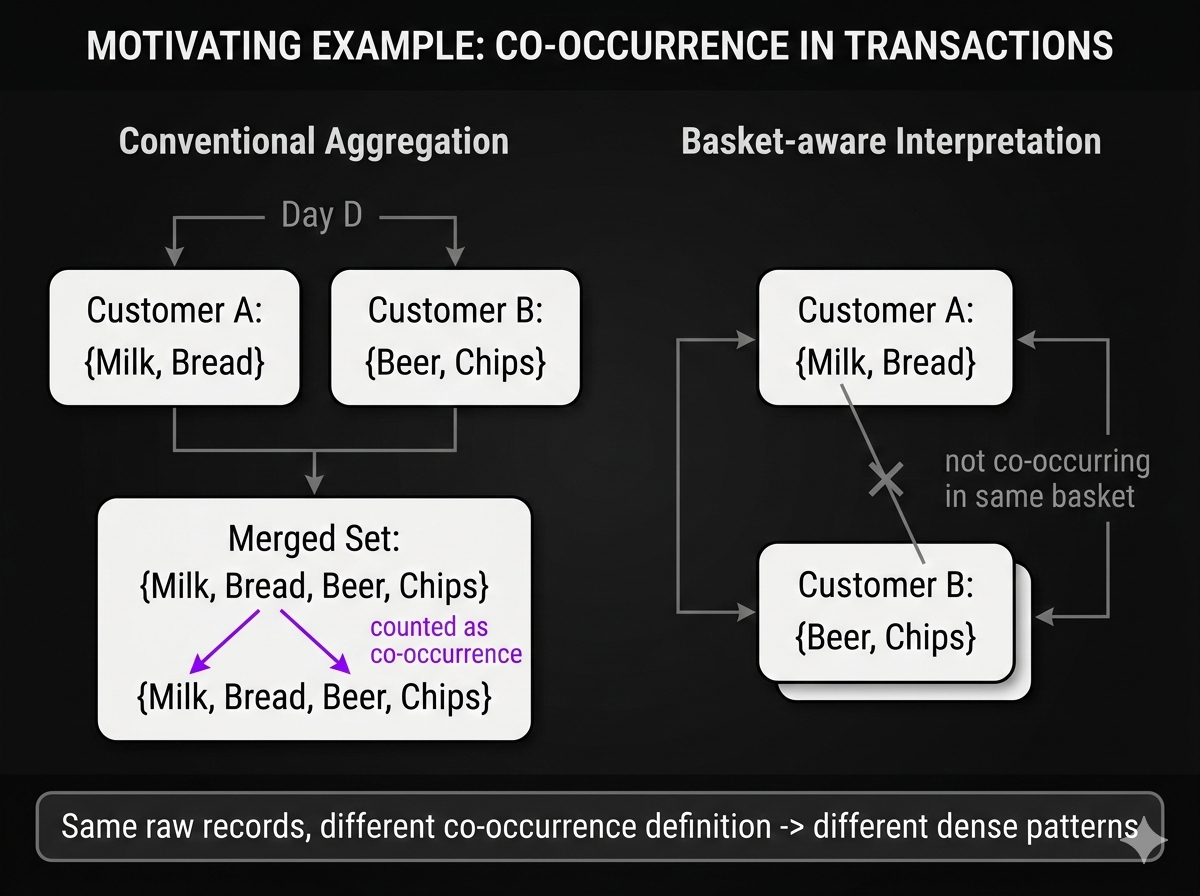
\includegraphics[width=\linewidth]{fig/motivating_example.png}
    \caption{偽共起の動機付け例}
    \label{fig:motivating}
\end{figure}

例えば，同日に顧客 A が \{牛乳, パン\}，顧客 B が \{ビール, ポテチ\} を購入した場合を考える．
日付単位で統合された 1 トランザクションをそのまま扱うと，
(牛乳, ビール) のような実際には同一購買イベントで共起していない組合せが
頻出として抽出され得る．この誤検出は，下流の需要予測や販促施策に
誤った示唆を与える．

本研究の位置づけは，DSAA2025 の枠組みを否定することではなく，
その有効性を維持したまま，未対応だった入力構造を拡張する点にある．
具体的には，共起の定義を「トランザクション内」から「バスケット内」へ変更した
Basket-aware Apriori-Window を提案する．
提案法の主貢献は以下の通りである．

\begin{itemize}
    \item \textbf{課題の明確化}: DSAA2025 の単一バスケット前提が，
    複数バスケット記録データにおいて偽共起を生む構造的要因であることを
    形式的に定義し，その影響を定量的に示す（\S\ref{sec:problem_def}）．

    \item \textbf{手法拡張と理論保証}: Apriori-window の枠組みを保ったまま，
    バスケット内共起に基づく探索へ拡張する．
    偽共起パターン率 SPR = 0 の理論保証（命題~\ref{prop:spr_zero}），
    バスケット内共起における反単調性の成立（定理~\ref{thm:anti_monotone}），
    および時間・空間計算量の解析（定理~\ref{thm:complexity}）を与える（\S\ref{sec:proposed_method}）．

    \item \textbf{合成データによる系統的評価}: Oracle 完全一致（E0），
    バスケット密度 sweep での偽共起爆発と完全排除（E1），
    構造パラメータへの頑健性（E2），
    大規模データでの計算優位（E3），
    区間品質の優位（E4）を確認する（\S\ref{sec:experiments}）．

    \item \textbf{実データによる外的妥当性}: 3 つの実データ
    （dunnhumby / onlineretail / chicago）で，
    従来法パターンの 74--99\% が偽共起であることを実証する（\S\ref{sec:exp_e6}）．
\end{itemize}

以上より，本稿は DSAA2025 の問題設定を現実のデータ構造へ拡張する
第一段階として，密集パターン抽出の信頼性向上に寄与する．
